% ============================================================
% BTL MAD 2026 - Báo Cáo Cá Nhân: Nguyễn Việt Huy - B22DCCN393
% Phạm vi: API Gateway & Identity Service
% ============================================================
\documentclass[14pt,a4paper,oneside]{extreport}

% ---- Encoding & Font ----
\usepackage{iftex}
\ifPDFTeX
  \usepackage[utf8]{inputenc}
  \usepackage[T5]{fontenc}
  \usepackage[vietnamese]{babel}
  \usepackage{times}              % Times New Roman
\else
  \usepackage{fontspec}
  \usepackage[vietnamese]{babel}
  \setmainfont{Times New Roman}
\fi

% ---- Geometry ----
\usepackage[
  top=2.5cm,
  bottom=2.5cm,
  left=3cm,
  right=2cm
]{geometry}

% ---- Packages ----
\usepackage{graphicx}
\usepackage{float}
\usepackage{array}
\usepackage{booktabs}
\usepackage{longtable}
\usepackage{tabularx}
\usepackage{enumitem}
\usepackage{hyperref}
\usepackage{xcolor}
\usepackage{fancyhdr}
\usepackage{titlesec}
\usepackage{caption}
\usepackage{indentfirst}
\usepackage{setspace}
\usepackage{listings}
\usepackage{tikz}

\newcommand{\coverpageborder}{%
  \begin{tikzpicture}[remember picture,overlay]
    \draw[line width=1.2pt]
      ([xshift=1.5cm,yshift=-1.5cm]current page.north west)
      rectangle
      ([xshift=-1.5cm,yshift=1.5cm]current page.south east);
    \draw[line width=0.4pt]
      ([xshift=1.65cm,yshift=-1.65cm]current page.north west)
      rectangle
      ([xshift=-1.65cm,yshift=1.65cm]current page.south east);
  \end{tikzpicture}%
}

% ---- Hyperref setup ----
\hypersetup{
  colorlinks=true,
  linkcolor=black,
  citecolor=black,
  urlcolor=blue
}

% ---- Spacing ----
\onehalfspacing
\setlength{\parindent}{1cm}

% ---- Header/Footer ----
\pagestyle{fancy}
\fancyhf{}
\fancyfoot[C]{\thepage}
\renewcommand{\headrulewidth}{0pt}

% ---- Chapter/Section Format ----
\titleformat{\chapter}[display]
  {\normalfont\Large\bfseries\centering}
  {\MakeUppercase{\chaptertitlename}\ \thechapter}{10pt}{\Large\MakeUppercase}
\titlespacing*{\chapter}{0pt}{-20pt}{20pt}

\titleformat{\section}
  {\normalfont\large\bfseries}{\thesection}{1em}{}
\titleformat{\subsection}
  {\normalfont\normalsize\bfseries}{\thesubsection}{1em}{}

% ---- Captions ----
\captionsetup{font=small, labelfont=bf}

% ---- Naming ----
\renewcommand{\listtablename}{Danh sách bảng biểu}
\renewcommand{\listfigurename}{Danh sách hình vẽ}
\renewcommand{\contentsname}{Mục lục}
\renewcommand{\chaptername}{Chương}
\renewcommand{\tablename}{Bảng}
\renewcommand{\figurename}{Hình}

% ---- Listings style ----
\lstset{
  basicstyle=\ttfamily\footnotesize,
  breaklines=true,
  frame=single,
  backgroundcolor=\color{gray!5},
  showstringspaces=false,
  numbers=none
}

% ============================================================
\begin{document}

% ============================================================
% TRANG BÌA (Tham khảo từ BTL_MAD_TV3_Gateway_Identity.tex)
% ============================================================
\begin{titlepage}
  \coverpageborder
  \begin{center}

    \textbf{\large HỌC VIỆN CÔNG NGHỆ BƯU CHÍNH VIỄN THÔNG}\\[2pt]
    \textbf{\large KHOA CÔNG NGHỆ THÔNG TIN}

    \vspace{0.35cm}

    
\includegraphics[width=2.4cm]{assets/logo_ptit.png}

    \vspace{0.45cm}

    {\large\textbf{BÁO CÁO BÀI TẬP LỚN CÁ NHÂN}}\\[6pt]
    {\Large\textbf{PHÁT TRIỂN ỨNG DỤNG CHO\\THIẾT BỊ DI ĐỘNG (MAD)}}

    \vspace{0.6cm}

    {\LARGE\textbf{PHÂN HỆ API GATEWAY \& IDENTITY SERVICE}}\\[6pt]
    {\large\textit{Hạ tầng kết nối và Quản lý danh tính người dùng ứng dụng Pody}}

    \vspace{1.0cm}

    \begin{tabular}{r l}
      \textbf{Giảng viên hướng dẫn:} & \textit{ThS. Nguyễn Hoàng Anh} \\[6pt]
      \textbf{Nhóm BTL:}             & \textit{01} \\[6pt]
      \textbf{Sinh viên thực hiện:}  & \textit{Nguyễn Việt Huy -- B22DCCN393} \\
    \end{tabular}

    \vspace{0.8cm}

    \textbf{Nhóm thành viên BTL chính:}

    \vspace{0.2cm}

    \begin{tabular}{|c|l|c|p{6.8cm}|}
      \hline
      \textbf{STT} & \textbf{Họ và tên} & \textbf{MSSV} & \textbf{Phân công chính} \\
      \hline
      1 & Lại Xuân Hiếu & B22DCCN309 & AI podcast (ai-service) \\
      \hline
      2 & Vũ Đức Thành & B22DCCN801 & Báo \& Embedding (article, embedding) \\
      \hline
      3 & \textbf{Nguyễn Việt Huy} & \textbf{B22DCCN393} & \textbf{Hạ tầng \& Auth (gateway, identity)} \\
      \hline
      4 & Lê Minh Ngọc & B22DCCN586 & Thông báo (notification-service) \\
      \hline
    \end{tabular}

    \vfill

    \textbf{Hà Nội, 2026}

  \end{center}
\end{titlepage}

% ============================================================
% MỤC LỤC
% ============================================================
\newpage
\tableofcontents

\newpage
\listoffigures
\listoftables

% ============================================================
% CHƯƠNG 1: DANH SÁCH CHỨC NĂNG ĐƯỢC PHÂN CÔNG
% ============================================================
\chapter{DANH SÁCH CHỨC NĂNG ĐƯỢC PHÂN CÔNG}
\label{chap:danh-sach-chuc-nang}

Trong phạm vi đề tài bài tập lớn, phân hệ \textbf{API Gateway} và \textbf{Identity Service} được phân công thực hiện với các chức năng chi tiết như sau:

\section{Phân hệ API Gateway (Cổng kết nối hệ thống)}
\begin{itemize}[leftmargin=1.5cm]
  \item \textbf{Định tuyến động (Dynamic Routing):} Xây dựng cổng truy cập HTTP tập trung tại cổng \texttt{8080}, cấu hình reverse proxy chuyển tiếp yêu cầu đến các microservices nội bộ tương ứng dựa trên tiền tố của đường dẫn (Path Prefix).
  \item \textbf{Cơ chế phân tách phân quyền (Public/Protected Routes):} Thiết lập bộ lọc router để phân tách rõ ràng các API công khai cho phép khách truy cập tự do (\texttt{/api/v1/public/*}) và các API bảo mật (\texttt{/api/v1/*}) yêu cầu người dùng phải xác thực.
  \item \textbf{Xác thực mã thông báo JWT (JWT Authentication Middleware):} Thiết lập bộ lọc chặn (intercept) tất cả request gửi vào các protected routes, giải mã và kiểm tra tính hợp lệ chữ ký của Access Token gửi kèm ở header.
  \item \textbf{Làm phong phú thông tin Request (Header Enrichment):} Trích xuất định danh người dùng (\texttt{user\_id}) và quyền hạn từ token đã giải mã, đính kèm vào tiêu đề HTTP (\texttt{X-Auth-User-ID}) để gửi sang các microservices downstream.
  \item \textbf{Cơ chế ghi nhận và truy vết (Request Tracing):} Tự động sinh mã duy nhất \texttt{Request-ID} cho mỗi yêu cầu kết nối, ghi log tập trung để hỗ trợ giám sát và gỡ lỗi xuyên suốt hệ thống microservices.
  \item \textbf{Hỗ trợ Trang cầu nối ứng dụng di động (Deep Link Bridges):} Tạo các trang web HTML trung gian tĩnh tại Gateway để xử lý điều hướng sâu (Deep Linking) cho các tác vụ kích hoạt tài khoản hoặc đặt lại mật khẩu từ liên kết email chuyển hướng vào ứng dụng Mobile.
\end{itemize}

\section{Phân hệ Identity Service (Quản lý danh tính người dùng)}
\begin{itemize}[leftmargin=1.5cm]
  \item \textbf{Đăng ký tài khoản (User Sign-up):} Cho phép đăng ký bằng email và mật khẩu. Mã hóa một chiều mật khẩu bằng thuật toán \texttt{bcrypt} có độ muối cao trước khi lưu vào CSDL.
  \item \textbf{Xác minh tài khoản qua Email (Email Verification):} Sinh mã token ngẫu nhiên dạng mã băm bảo mật gửi qua hộp thư điện tử của người dùng. Kích hoạt tài khoản khi mã khớp và còn hiệu lực.
  \item \textbf{Đăng nhập truyền thống (Email/Password Sign-in):} Kiểm tra thông tin xác thực, sinh và trả về bộ đôi mã thông báo Access Token (thời hạn 15 phút) và Refresh Token (thời hạn 30 ngày).
  \item \textbf{Đăng nhập liên kết bên thứ ba (Google Sign-In OAuth2):} Tiếp nhận ID Token từ client, tích hợp trực tiếp với dịch vụ Google API để kiểm chứng danh tính của người dùng, tự động khởi tạo hồ sơ nếu là lần đầu truy cập.
  \item \textbf{Quản lý phiên làm việc và Làm mới phiên (Refresh Token Rotation):} Lưu thông tin băm của Refresh Token vào bảng quản lý phiên hoạt động. Hỗ trợ cơ chế luân phiên cấp mới mã thông báo để bảo vệ chống giả mạo phiên.
  \item \textbf{Khôi phục và Đặt lại mật khẩu (Forgot/Reset Password):} Tiếp nhận yêu cầu quên mật khẩu, sinh mã xác thực OTP dùng một lần (One-Time Password) gửi qua email, kiểm tra tính hợp lệ và cho phép đặt lại mật khẩu mới đồng thời thu hồi mọi phiên làm việc hiện hành.
  \item \textbf{Quản lý thông tin hồ sơ và Ảnh đại diện (Profile \& Avatar Upload):} Cung cấp API cập nhật thông tin cá nhân của người dùng hiện tại, tích hợp với API ngoài của dịch vụ Supabase Storage để lưu trữ và lấy đường dẫn ảnh đại diện.
\end{itemize}

% ============================================================
% CHƯƠNG 2: KIẾN TRÚC CHI TIẾT HỆ THỐNG
% ============================================================
\chapter{KIẾN TRÚC CHI TIẾT HỆ THỐNG}
\label{chap:kien-truc-chi-tiet}

\section{Mô hình thành phần chi tiết (Component Diagram)}
Kiến trúc của phân hệ hạ tầng được thiết kế nhằm mục đích đảm bảo tính độc lập giữa các thành phần nghiệp vụ, giảm thiểu sự liên kết cứng (loose coupling) và tối ưu hóa hiệu năng phản hồi. Sơ đồ các thành phần chi tiết của API Gateway và Identity Service cùng các mối quan hệ được biểu diễn trong Hình~\ref{fig:component-huy}.

\begin{figure}[H]
  \centering
  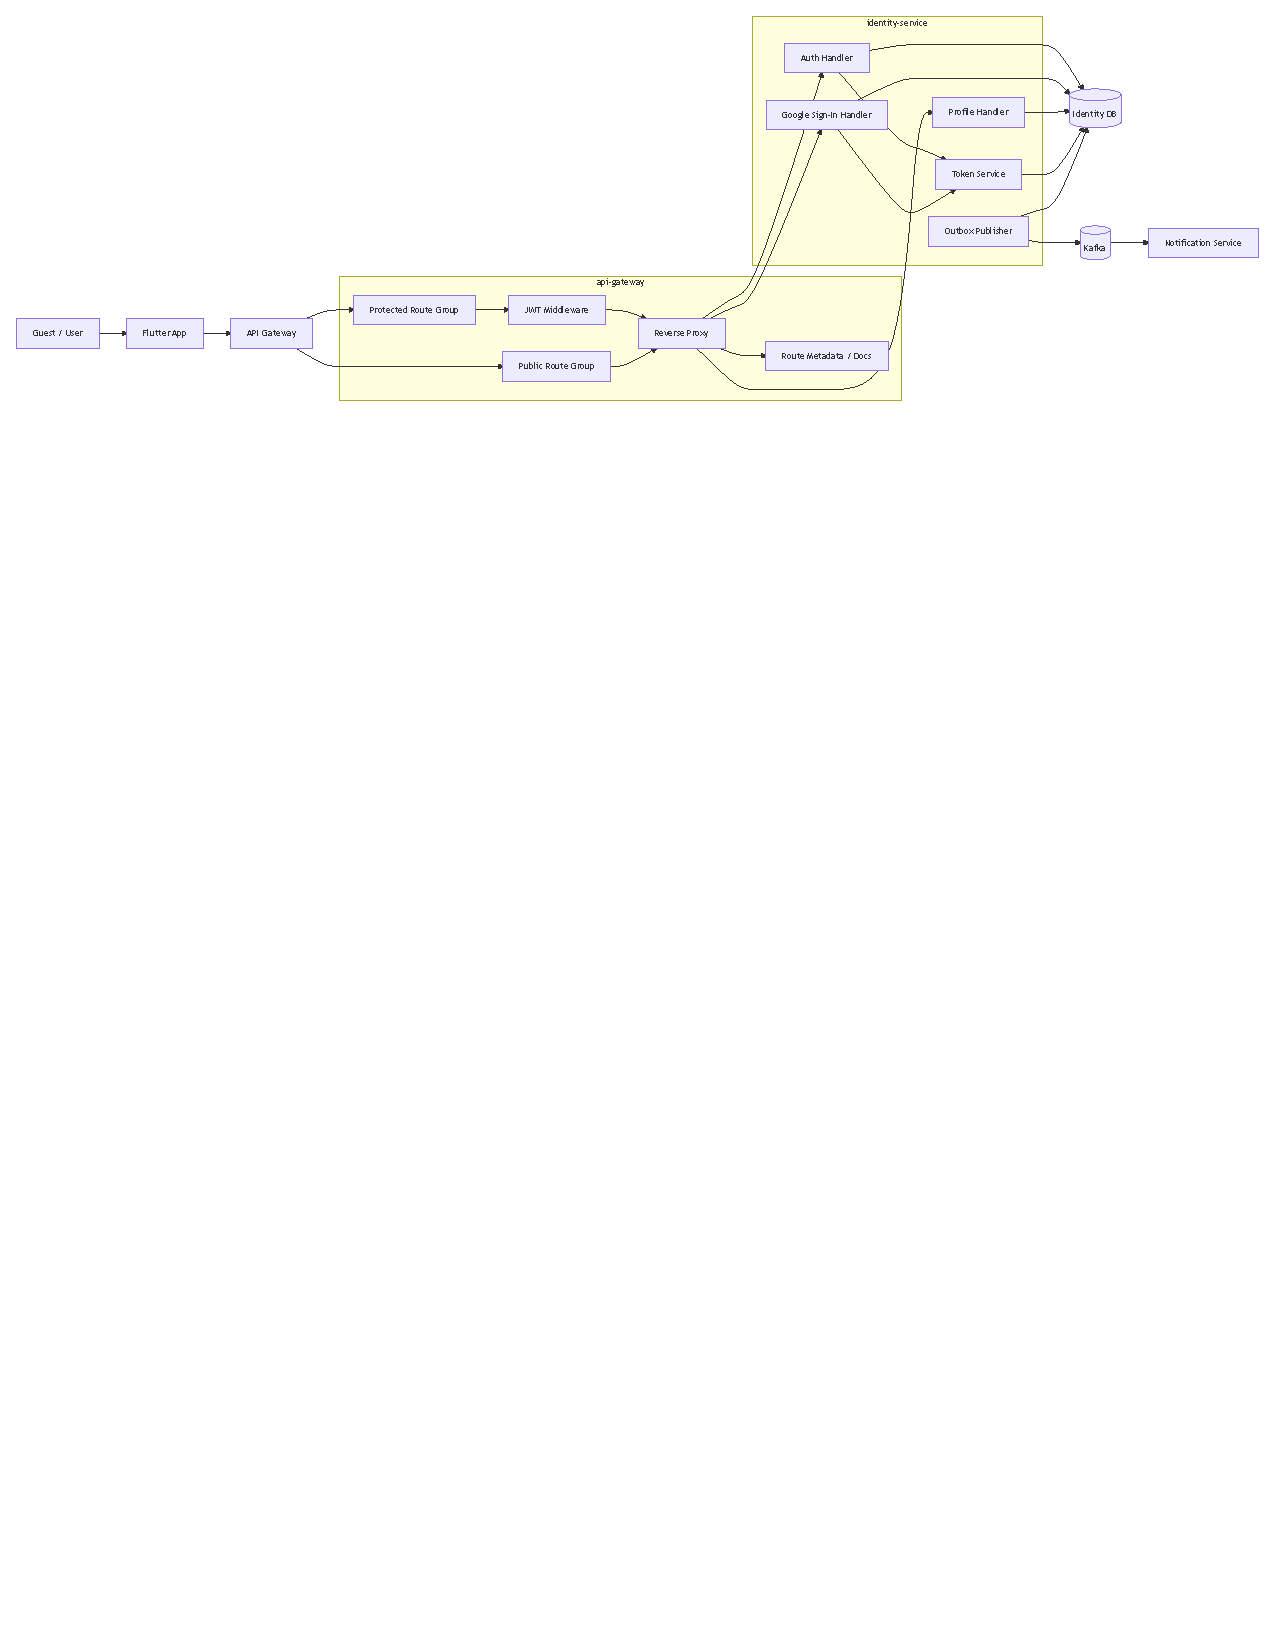
\includegraphics[width=\textwidth,height=0.65\textheight,keepaspectratio]{diagrams/component_identity_gateway.pdf}
  \caption{Sơ đồ Component phân hệ API Gateway và Identity Service}
  \label{fig:component-huy}
\end{figure}

Các thành phần cấu thành chính bao gồm:
\begin{itemize}[leftmargin=1.5cm]
  \item \textbf{Flutter Mobile Client:} Điểm đầu tiếp xúc với người dùng, kết nối tới API Gateway qua giao thức HTTP REST.
  \item \textbf{API Gateway (Go / Chi Router):} Nhận request, xử lý CORS, phân luồng theo route, kiểm tra chữ ký token JWT qua middleware. Sử dụng \texttt{ReverseProxy} của ngôn ngữ Go để chuyển tiếp yêu cầu đến các microservices nằm trong mạng nội bộ.
  \item \textbf{Identity Service (Go):} Nhận request nội bộ, thực thi logic đăng ký, đăng nhập, quản lý phiên và hồ sơ cá nhân.
  \item \textbf{Identity Database (PostgreSQL):} Hệ quản trị CSDL quan hệ lưu trữ độc lập dữ liệu người dùng, token và phiên làm việc.
  \item \textbf{Apache Kafka Message Broker:} Đóng vai trò là kênh truyền tin bất đồng bộ. Identity Service sử dụng cơ chế Transactional Outbox ghi tin nhắn vào DB rồi đẩy lên Kafka nhằm tránh việc thất thoát sự kiện khi xảy ra lỗi mạng.
\end{itemize}

\section{Cơ chế kết nối và tương tác giữa các thành phần}
Sự tương tác giữa các thành phần diễn ra qua hai hình thức chính:

\subsection{Tương tác đồng bộ (Synchronous Interaction via HTTP/REST)}
Sử dụng cho các thao tác yêu cầu kết quả phản hồi tức thời từ hệ thống (Đăng ký, Đăng nhập, Truy vấn Profile, Đổi avatar).
\begin{enumerate}[leftmargin=1.5cm]
  \item Client gửi HTTP request chứa Access Token trong header \texttt{Authorization:\allowbreak\ Bearer\allowbreak\ <token>} đến Gateway.
  \item Gateway chặn request, kiểm tra định dạng và verify chữ ký số của token bằng khóa bí mật chung (\texttt{JWT\_SECRET}). Nếu không hợp lệ, trả ngay mã lỗi \texttt{401 Unauthorized}.
  \item Nếu token hợp lệ, Gateway trích xuất trường \texttt{user\allowbreak\_id} từ token payload, ghi đè vào request header \texttt{X-Auth-\allowbreak User-ID} và chuyển tiếp (forward) request đến cổng nội bộ của \texttt{identity-\allowbreak service}.
  \item \texttt{identity-\allowbreak service} nhận request, đọc thông tin từ header \texttt{X-Auth-\allowbreak User-ID} để định danh người dùng và truy vấn thông tin cần thiết từ Identity Database để trả về kết quả.
\end{enumerate}

\subsection{Tương tác bất đồng bộ (Asynchronous Interaction via Transactional Outbox \& Kafka)}
Sử dụng cho các hành vi nghiệp vụ cần thông báo cho phân hệ khác xử lý mà không cần client phải đợi phản hồi tức thời (gửi email xác minh tài khoản, gửi OTP khôi phục mật khẩu).
\begin{enumerate}[leftmargin=1.5cm]
  \item \textbf{Lưu trữ giao dịch nhất quán:} Khi có sự kiện (ví dụ: đăng ký tài khoản), trong cùng một Database Transaction, \texttt{identity-\allowbreak service} tiến hành chèn thông tin user mới vào bảng \texttt{users} và chèn bản ghi mô tả sự kiện vào bảng \texttt{outbox\allowbreak\_events}.
  \item \textbf{Đẩy tin nhắn ngầm (Outbox Publisher):} Một tiến trình chạy nền độc lập (\texttt{OutboxPublisher}) thực hiện quét bảng \texttt{outbox\allowbreak\_events} định kỳ với chu kỳ ngắn (100ms) để lấy các sự kiện chưa gửi, đóng gói và phát (publish) lên Kafka topic \texttt{identity-\allowbreak events}.
  \item \textbf{Dọn dẹp sự kiện đã gửi (Outbox Cleanup):} Sau khi nhận được tín hiệu phản hồi xác nhận gửi thành công từ Kafka broker, bản ghi sự kiện trong outbox được đánh dấu là đã gửi thành công. Tiến trình \texttt{OutboxCleanup} chạy ngầm định kỳ quét và xóa các bản ghi sự kiện đã gửi thành công cũ để làm gọn CSDL.
  \item \textbf{Tiêu thụ sự kiện downstream (Notification Consumer):} Phân hệ \texttt{notification-\allowbreak service} lắng nghe topic Kafka này, đọc thông tin sự kiện, gọi dịch vụ gửi thư SMTP để chuyển email kích hoạt hoặc OTP đến hòm thư của người dùng.
\end{enumerate}

% ============================================================
% CHƯƠNG 3: MÃ NGUỒN VÀ DỮ LIỆU ĐÁP ỨNG CHỨC NĂNG
% ============================================================
\chapter{MÃ NGUỒN VÀ DỮ LIỆU ĐÁP ỨNG CHỨC NĂNG}
\label{chap:code-va-du-lieu}

\section{Cấu trúc các bảng dữ liệu trong CSDL (Database Schemas)}
Identity DB sử dụng hệ quản trị cơ sở dữ liệu PostgreSQL. Sơ đồ thực thể liên kết (ER Diagram) cho các bảng thuộc phân hệ được biểu diễn trong Hình~\ref{fig:er-huy}.

\begin{figure}[H]
  \centering
  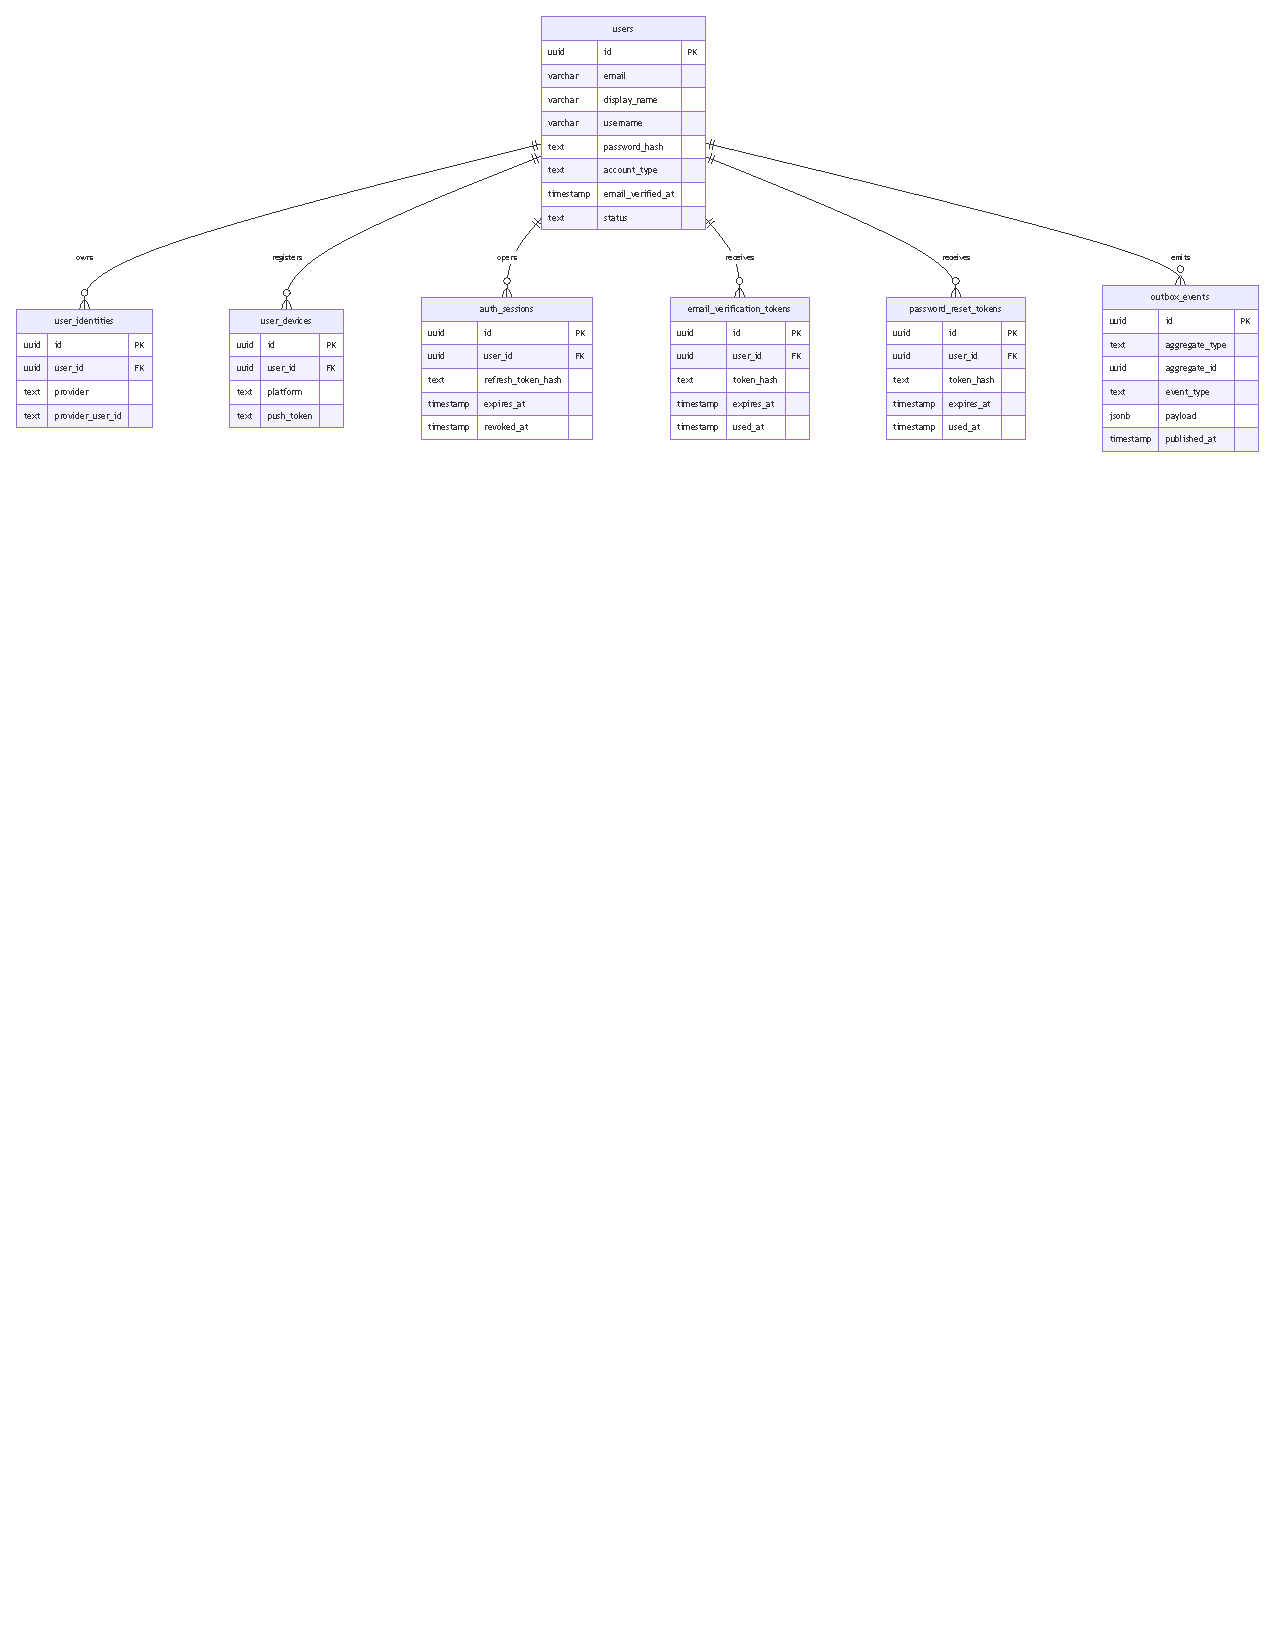
\includegraphics[width=\textwidth,height=0.60\textheight,keepaspectratio]{diagrams/er_identity.pdf}
  \caption{Sơ đồ thực thể liên kết (ER) của Identity Database}
  \label{fig:er-huy}
\end{figure}

Chi tiết cấu trúc và ý nghĩa của các bảng cơ sở dữ liệu như sau:

\subsection{Bảng \texttt{users}}
Lưu trữ thông tin định danh gốc của người dùng hệ thống.
\begin{itemize}[leftmargin=1.5cm]
  \item \texttt{id}: UUID (Primary Key) -- Khóa chính tự sinh định danh duy nhất của người dùng.
  \item \texttt{email}: VARCHAR(255) (Unique) -- Địa chỉ thư điện tử dùng để đăng nhập.
  \item \texttt{username}: VARCHAR(50) (Unique, Nullable) -- Tên tài khoản hiển thị hệ thống.
  \item \texttt{password\allowbreak\_hash}: VARCHAR(255) (Nullable) -- Mật khẩu đã được mã hóa băm bcrypt một chiều. Trường này rỗng nếu tài khoản đăng nhập trực tiếp qua liên kết Google.
  \item \texttt{display\allowbreak\_name}: VARCHAR(100) -- Tên hiển thị công khai trên ứng dụng.
  \item \texttt{avatar\allowbreak\_url}: VARCHAR(500) (Nullable) -- Liên kết đến tệp ảnh đại diện được lưu trữ trên Supabase Storage.
  \item \texttt{status}: VARCHAR(20) -- Trạng thái tài khoản (ví dụ: \texttt{pending\_}\allowbreak\texttt{verification}, \texttt{active}, \texttt{suspended}).
  \item \texttt{account\allowbreak\_type}: VARCHAR(20) -- Loại tài khoản (\texttt{email}, \texttt{google}).
  \item \texttt{locale}: VARCHAR(5) -- Thiết lập ngôn ngữ mặc định (\texttt{vi}, \texttt{en}).
  \item \texttt{email\allowbreak\_verified\allowbreak\_at}: TIMESTAMP -- Thời gian xác minh thư điện tử thành công.
\end{itemize}

\subsection{Bảng \texttt{user\_identities}}
Quản lý các tài khoản liên kết đăng nhập bên thứ ba (Google OAuth2).
\begin{itemize}[leftmargin=1.5cm]
  \item \texttt{id}: BIGSERIAL (Primary Key) -- Khóa chính tự tăng.
  \item \texttt{user\allowbreak\_id}: UUID (Foreign Key) -- Tham chiếu liên kết đến bảng \texttt{users.id}.
  \item \texttt{provider}: VARCHAR(50) -- Tên nhà cung cấp xác thực (\texttt{google}).
  \item \texttt{provider\allowbreak\_user\allowbreak\_id}: VARCHAR(255) -- Khóa ID định danh duy nhất của người dùng do Google cung cấp.
\end{itemize}

\subsection{Bảng \texttt{auth\_sessions}}
Quản lý các phiên đăng nhập đang hoạt động và hỗ trợ thu hồi quyền truy cập (Sign-out / Revoke session).
\begin{itemize}[leftmargin=1.5cm]
  \item \texttt{id}: UUID (Primary Key) -- Mã định danh phiên làm việc.
  \item \texttt{user\allowbreak\_id}: UUID (Foreign Key) -- Tham chiếu liên kết đến bảng \texttt{users.id}.
  \item \texttt{refresh\allowbreak\_token\allowbreak\_hash}: VARCHAR(255) -- Mã băm bảo mật SHA256 của Refresh Token tương ứng nhằm bảo vệ chống lộ mã thông báo dưới dạng văn bản rõ.
  \item \texttt{expires\allowbreak\_at}: TIMESTAMP -- Thời hạn phiên đăng nhập hết hiệu lực.
  \item \texttt{is\allowbreak\_revoked}: BOOLEAN -- Trạng thái đã thu hồi phiên truy cập (mặc định là \texttt{false}).
\end{itemize}

\subsection{Bảng \texttt{email\_verification\_tokens}}
Lưu giữ mã băm dùng để xác thực hòm thư điện tử.
\begin{itemize}[leftmargin=1.5cm]
  \item \texttt{id}: BIGSERIAL (Primary Key) -- Khóa chính.
  \item \texttt{user\allowbreak\_id}: UUID (Foreign Key) -- Liên kết đến bảng \texttt{users.id}.
  \item \texttt{token\allowbreak\_hash}: VARCHAR(255) -- Mã xác thực băm SHA256 gửi qua email.
  \item \texttt{expires\allowbreak\_at}: TIMESTAMP -- Hạn hết hiệu lực của mã xác thực (24 giờ).
\end{itemize}

\subsection{Bảng \texttt{password\_reset\_tokens}}
Lưu trữ mã OTP bảo mật để phục vụ khôi phục đặt lại mật khẩu.
\begin{itemize}[leftmargin=1.5cm]
  \item \texttt{id}: BIGSERIAL (Primary Key) -- Khóa chính.
  \item \texttt{user\allowbreak\_id}: UUID (Foreign Key) -- Liên kết đến bảng \texttt{users.id}.
  \item \texttt{token\allowbreak\_hash}: VARCHAR(255) -- Mã OTP băm dùng một lần.
  \item \texttt{expires\allowbreak\_at}: TIMESTAMP -- Thời điểm mã OTP hết hạn (15 phút).
\end{itemize}

\subsection{Bảng \texttt{outbox\_events}}
Lưu trữ tạm các sự kiện phát sinh từ hệ thống Identity trước khi đẩy lên Kafka.
\begin{itemize}[leftmargin=1.5cm]
  \item \texttt{id}: UUID (Primary Key) -- Khóa chính định danh sự kiện.
  \item \texttt{aggregate\allowbreak\_type}: VARCHAR(50) -- Loại thực thể gây ra sự kiện (\texttt{user}).
  \item \texttt{aggregate\allowbreak\_id}: VARCHAR(255) -- Khóa định danh của thực thể liên quan (\texttt{user\allowbreak\_id}).
  \item \texttt{event\allowbreak\_type}: VARCHAR(100) -- Tên sự kiện (ví dụ: \texttt{UserRegistered}, \allowbreak \texttt{PasswordResetRequested}, \allowbreak \texttt{UserUpdated}).
  \item \texttt{payload}: JSONB -- Nội dung dữ liệu chi tiết của sự kiện.
  \item \texttt{status}: VARCHAR(20) -- Trạng thái gửi tin (ví dụ: \texttt{pending}, \allowbreak \texttt{published}, \allowbreak \texttt{failed}).
  \item \texttt{attempts}: INTEGER -- Số lần đã thử gửi tin nhắn lên broker.
  \item \texttt{last\allowbreak\_error}: TEXT -- Nội dung lỗi kỹ thuật ở lần thử gửi gần nhất.
\end{itemize}

\section{Bản đồ ánh xạ mã nguồn đáp ứng chức năng (Code Mapping)}
Toàn bộ mã nguồn backend của cụm Gateway và Identity Service được viết bằng ngôn ngữ lập trình Go. Bảng~\ref{tab:code-map-detail} mô tả cụ thể sự liên kết giữa các chức năng nghiệp vụ với các tệp tin mã nguồn, cấu trúc dữ liệu và các hàm tương ứng.

\begin{table}[H]
\centering
\caption{Bản đồ ánh xạ các chức năng và mã nguồn liên quan}
\label{tab:code-map-detail}
\renewcommand{\arraystretch}{1.2}
\scriptsize
\begin{tabularx}{\textwidth}{|>{\raggedright\arraybackslash}p{2.5cm}|>{\hsize=0.8\hsize\raggedright\arraybackslash}X|>{\hsize=1.2\hsize\raggedright\arraybackslash}X|}
\hline
\textbf{Chức năng phân công} & \textbf{Lớp / Hàm nghiệp vụ} & \textbf{Tệp nguồn liên quan và Giải thích} \\
\hline
\textbf{Reverse Proxy} &
  \texttt{httpserver.\allowbreak newServiceProxy} \newline
  \texttt{httpserver.\allowbreak joinPaths} &
  \texttt{api-gateway/internal/} \newline \texttt{httpserver/proxy.go} \newline
  Định tuyến và proxy request, xử lý ghi đè và cắt bỏ tiền tố API để chuyển đổi URL trước khi gọi hạ tầng downstream. \\
\hline
\textbf{Xác thực JWT} &
  \texttt{httpserver.\allowbreak withJWTAuth} \newline
  \texttt{httpserver.\allowbreak enrichRequestWithClaims} &
  \texttt{api-gateway/internal/} \newline \texttt{httpserver/middleware.go} \newline
  Bộ lọc middleware giải mã token JWT bằng khóa bí mật chung, kiểm tra chữ ký và trích xuất claims gán vào request headers. \\
\hline
\textbf{Đăng ký tài khoản} &
  \texttt{AuthService.\allowbreak SignUp} \newline
  \texttt{PostgresStore.\allowbreak CreateUserWithEmail} &
  \texttt{identity-service/internal/} \newline \texttt{auth/service.go} \newline
  \texttt{identity-service/internal/} \newline \texttt{store/postgres.go} \newline
  Mã hóa bcrypt mật khẩu, chèn bản ghi user trạng thái chờ xác minh kèm tạo outbox event trong cùng một Transaction CSDL. \\
\hline
\textbf{Đăng nhập tài khoản} &
  \texttt{AuthService.\allowbreak SignIn} \newline
  \texttt{PostgresStore.\allowbreak CreateSession} &
  \texttt{identity-service/internal/} \newline \texttt{auth/service.go} \newline
  Đối sánh mật khẩu đã băm, cấp bộ Access/Refresh Token và lưu hash Refresh Token vào bảng session để theo dõi. \\
\hline
\textbf{Google Sign-In} &
  \texttt{AuthService.\allowbreak SignInWithGoogle} \newline
  \texttt{googleauth.\allowbreak VerifyToken} &
  \texttt{identity-service/internal/} \newline \texttt{auth/service.go} \newline
  \texttt{identity-service/internal/} \newline \texttt{googleauth/google.go} \newline
  Gọi API ngoài của Google để xác thực ID Token nhận từ ứng dụng di động, đồng bộ thông tin tài khoản người dùng tương ứng. \\
\hline
\textbf{Quản lý Ảnh đại diện} &
  \texttt{httpserver.\allowbreak server.\allowbreak updateAvatar} \newline
  \texttt{storage.\allowbreak SupabaseStorage.\allowbreak UploadAvatar} &
  \texttt{identity-service/internal/} \newline \texttt{httpserver/server.go} \newline
  \texttt{identity-service/internal/} \newline \texttt{media/supabase.go} \newline
  Nhận file ảnh tải lên, tích hợp API ngoài của Supabase qua HTTP Client tải ảnh lên Bucket và cập nhật URL ảnh vào CSDL. \\
\hline
\textbf{Làm mới phiên} &
  \texttt{AuthService.\allowbreak RefreshToken} \newline
  \texttt{tokens.\allowbreak GenerateTokenPair} &
  \texttt{identity-service/internal/} \newline \texttt{auth/service.go} \newline
  Verify Refresh Token gửi từ client, thu hồi phiên đăng nhập cũ trong CSDL và phát hành bộ mã thông báo mới thay thế. \\
\hline
\textbf{Quên \& Đặt lại mật khẩu} &
  \texttt{AuthService.\allowbreak ForgotPassword} \newline
  \texttt{AuthService.\allowbreak ResetPassword} &
  \texttt{identity-service/internal/} \newline \texttt{auth/service.go} \newline
  ForgotPassword sinh mã OTP gửi qua outbox. ResetPassword kiểm tra mã OTP, cập nhật mật khẩu đã băm bcrypt và revoke mọi phiên làm việc cũ. \\
\hline
\textbf{Đẩy tin nhắn ngầm} &
  \texttt{outbox.\allowbreak Publisher.\allowbreak Start} \newline
  \texttt{outbox.\allowbreak Cleanup.\allowbreak Start} &
  \texttt{identity-service/internal/} \newline \texttt{outbox/publisher.go} \newline
  Tiến trình chạy ngầm quét bảng outbox định kỳ, đẩy dữ liệu JSON sự kiện lên Kafka Broker và thực hiện dọn dẹp các bản ghi cũ. \\
\hline
\end{tabularx}
\end{table}

\section{Tích hợp với dịch vụ bên thứ ba (External APIs)}
Phân hệ hạ tầng tích hợp hai API bên thứ ba để đảm bảo các tính năng hoạt động an toàn và phong phú:

\subsection{Google OAuth2 API (https://oauth2.googleapis.com/tokeninfo)}
\begin{itemize}[leftmargin=1.5cm]
  \item \textbf{Mục đích:} Hỗ trợ tính năng đăng nhập nhanh thông qua tài khoản Google bằng cách kiểm thực tính hợp lệ của thẻ định danh nhận được từ Client.
  \item \textbf{Cơ chế gọi:} Sử dụng thư viện HTTP client chuẩn của Go để tạo yêu cầu GET gửi lên API của Google kèm theo tham số truy vấn là ID Token của người dùng. Google API trả về cấu trúc JSON chứa các trường \texttt{email}, \texttt{name}, \texttt{picture} và \texttt{sub} (mã định danh người dùng duy nhất của Google). Hệ thống dựa vào đó để liên kết tài khoản.
\end{itemize}

\subsection{Supabase Storage REST API}
\begin{itemize}[leftmargin=1.5cm]
  \item \textbf{Mục đích:} Lưu trữ tập tin ảnh đại diện của người dùng công khai trên Internet.
  \item \textbf{Cơ chế gọi:} Sử dụng HTTP REST Client gửi request POST có định dạng payload là \texttt{multipart/form-data} đến endpoint lưu trữ của Supabase (\texttt{/storage/\allowbreak v1/\allowbreak object/\allowbreak avatars/}), đính kèm mã xác thực Authorization Bearer chứa API Key của dự án để tải file lên bucket, sau đó lấy về URL liên kết tĩnh để cập nhật vào cơ sở dữ liệu.
\end{itemize}

\section{Sơ đồ trình tự nghiệp vụ (Sequence Diagrams)}
Sự tương tác chi tiết giữa các phân hệ và thành phần mã nguồn được thể hiện rõ nét qua các sơ đồ trình tự dưới đây.

Hình~\ref{fig:seq-signup} mô tả chi tiết quy trình đăng ký tài khoản mới và xác minh qua thư điện tử. Có sự tham gia của Transactional Outbox để đảm bảo tính nhất quán dữ liệu giữa DB và Kafka:
\begin{figure}[H]
  \centering
  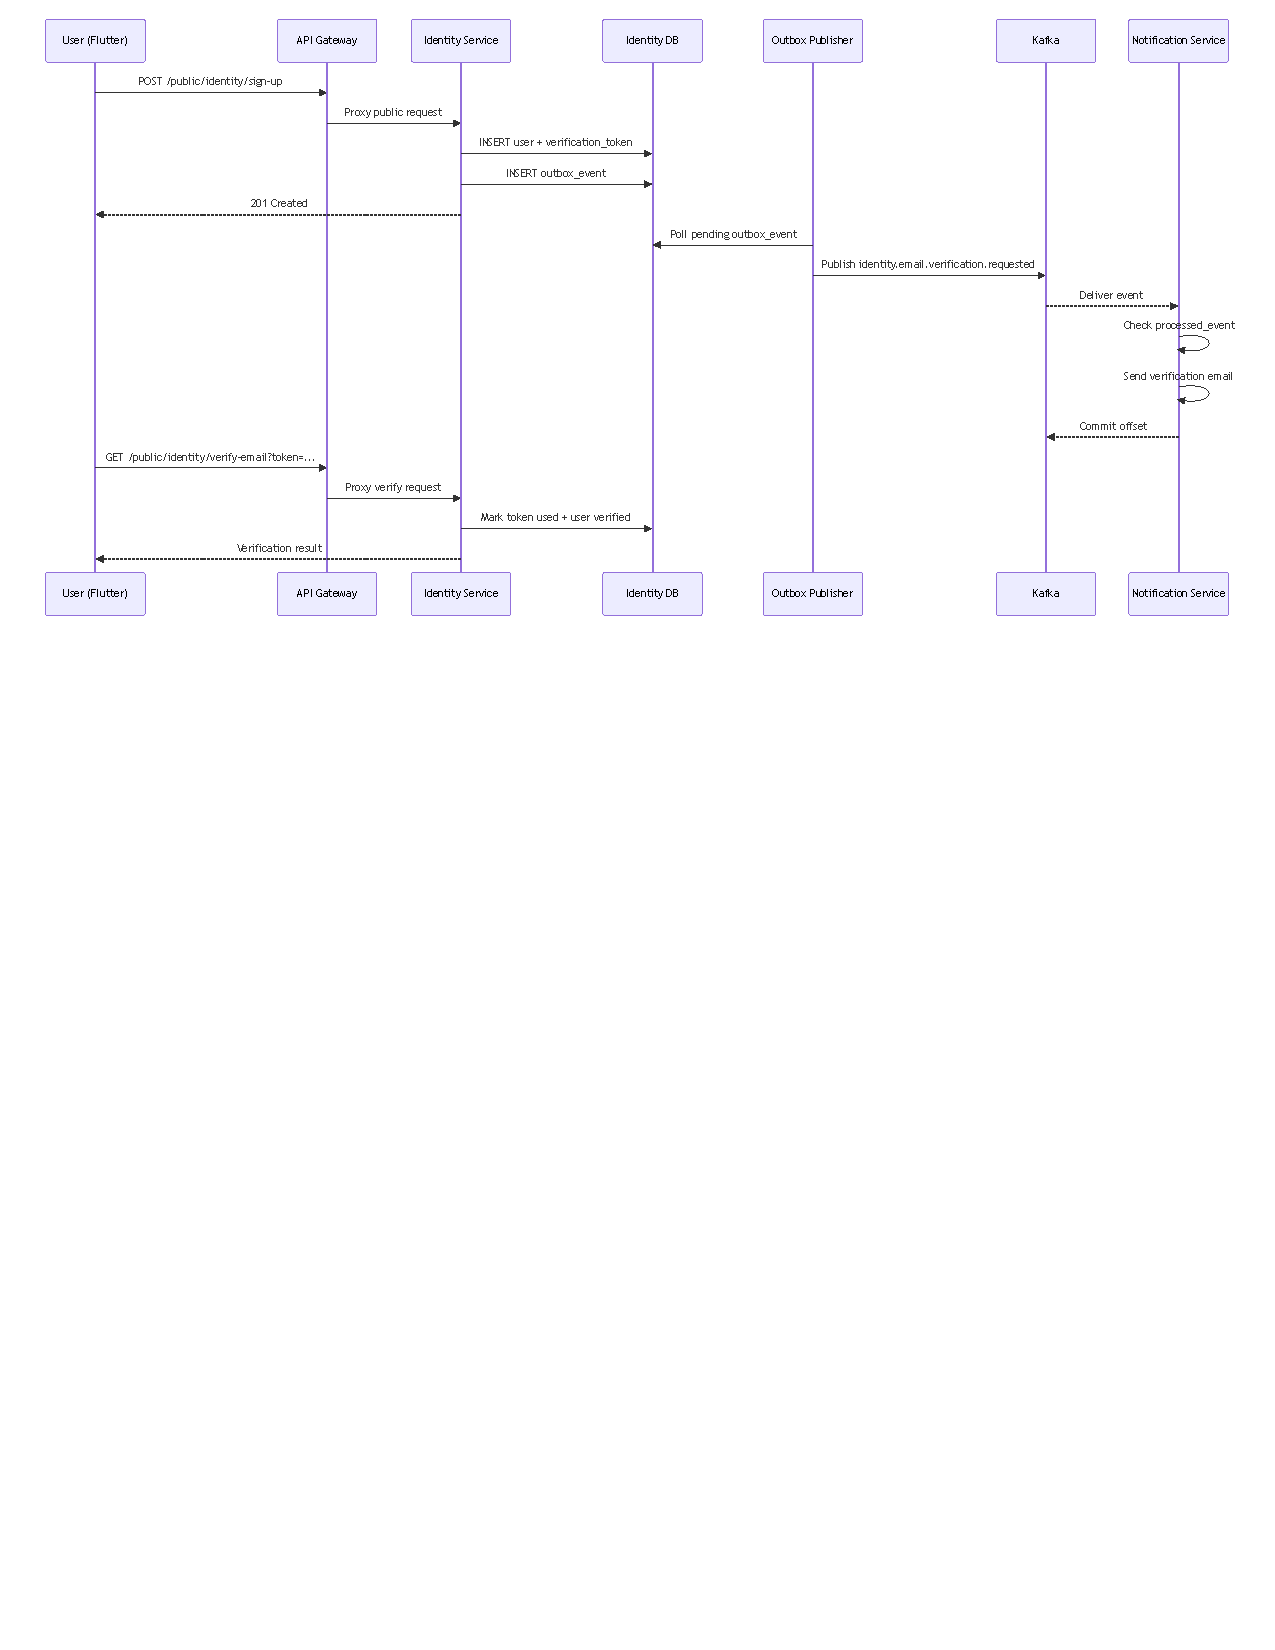
\includegraphics[width=\textwidth,height=0.72\textheight,keepaspectratio]{diagrams/seq_identity_signup_verify.pdf}
  \caption{Sơ đồ trình tự luồng đăng ký tài khoản và xác minh email}
  \label{fig:seq-signup}
\end{figure}

Hình~\ref{fig:seq-protected} mô tả quá trình API Gateway đóng vai trò là chốt chặn bảo mật, tiếp nhận các yêu cầu truy cập được bảo vệ và ủy quyền chuyển tiếp dữ liệu đến các service downstream:
\begin{figure}[H]
  \centering
  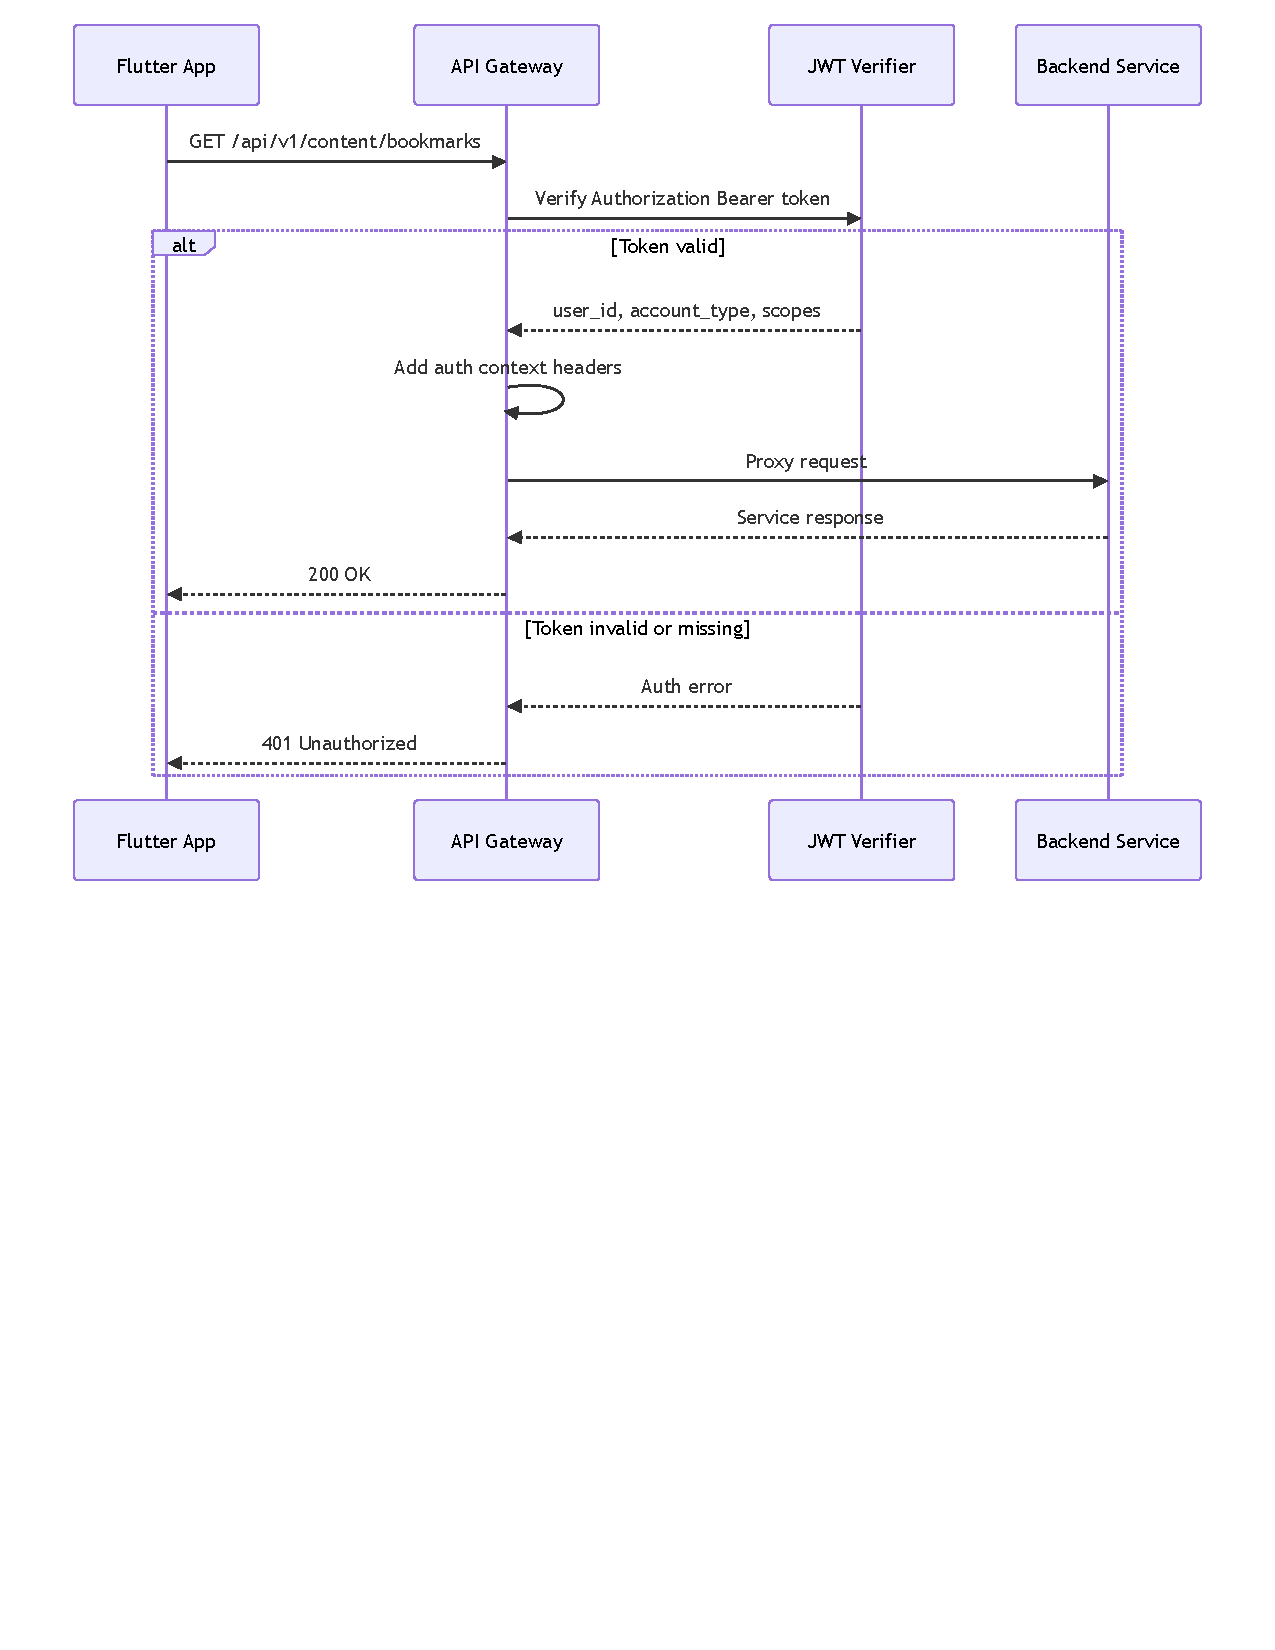
\includegraphics[width=\textwidth,height=0.72\textheight,keepaspectratio]{diagrams/seq_gateway_protected.pdf}
  \caption{Sơ đồ trình tự luồng gọi API bảo vệ qua API Gateway}
  \label{fig:seq-protected}
\end{figure}

% ============================================================
% CHƯƠNG 4: HƯỚNG DẪN VÀ CÁC LƯU Ý KHI CÀI ĐẶT TRIỂN KHAI
% ============================================================
\chapter{HƯỚNG DẪN VÀ CÁC LƯU Ý KHI CÀI ĐẶT TRIỂN KHAI}
\label{chap:huong-dan-trien-khai}

\section{Yêu cầu môi trường tối thiểu}
Để đảm bảo triển khai và vận hành hệ thống cục bộ (local) trơn tru, máy chủ phát triển cần chuẩn bị sẵn sàng cấu hình sau:
\begin{itemize}[leftmargin=1.5cm]
  \item \textbf{Phần cứng:} CPU tối thiểu 4 Cores, bộ nhớ trong RAM tối thiểu 16GB (khuyến nghị 24GB do chạy đồng thời nhiều database Postgres độc lập và Apache Kafka Broker).
  \item \textbf{Phần mềm:} Docker Desktop (phiên bản v4.20 trở lên) cài kèm Docker Compose CLI, Git Client.
  \item \textbf{Cổng mạng tự do:} Đảm bảo các cổng kết nối dịch vụ sau đây trên máy host chưa bị ứng dụng nào khác chiếm dụng trước khi bật container:
    \begin{itemize}
      \item \texttt{8080}: API Gateway (Cổng giao tiếp duy nhất ra ngoài).
      \item \texttt{8081}: Identity Service API nội bộ.
      \item \texttt{5433}: PostgreSQL instance chính (Article DB).
      \item \texttt{5434}: PostgreSQL instance phụ (Embedding DB).
      \item \texttt{6379}: Redis Cache.
      \item \texttt{8090}: Giao diện quản trị Kafka UI.
      \item \texttt{9000} \& \texttt{9001}: MinIO Console \& Storage API.
    \end{itemize}
\end{itemize}

\section{Quy trình các bước triển khai chi tiết}
Hệ thống Pody cung cấp các tệp Docker Compose cấu trúc riêng biệt để đơn giản hóa quá trình khởi chạy. Các bước thực hiện tuần tự như sau:

\subsection{Bước 1: Clone mã nguồn dự án}
Truy cập Terminal hoặc PowerShell, chạy lệnh sau để tải mã nguồn dự án về thư mục làm việc:
\begin{lstlisting}[language=bash]
git clone -b main https://github.com/pody-team/pody-app.git
cd pody-app
\end{lstlisting}

\subsection{Bước 2: Thiết lập cấu hình môi trường}
Tạo tệp cấu hình môi trường \texttt{.env} tại thư mục gốc của dự án. Khai báo các khóa bí mật cần thiết cho hệ thống:
\begin{lstlisting}[language=bash]
JWT_SECRET=your_jwt_secret_key_here
GOOGLE_CLIENT_ID=your_google_oauth2_client_id.apps.googleusercontent.com
SUPABASE_URL=https://your-project-id.supabase.co
SUPABASE_KEY=your-supabase-anon-key
SMTP_HOST=smtp.gmail.com
SMTP_PORT=587
SMTP_USER=your-email@gmail.com
SMTP_PASS=your-app-password
\end{lstlisting}

\subsection{Bước 3: Khởi chạy tầng hạ tầng cơ sở (Infrastructure)}
Triển khai hệ quản trị CSDL PostgreSQL, Message Broker Kafka, Redis Cache và MinIO Storage trước bằng cách chạy lệnh:
\begin{lstlisting}[language=bash]
docker-compose -f docker-compose.infra.yml up -d
\end{lstlisting}
\textit{Lưu ý quan trọng:} Đợi khoảng 10-15 giây để Kafka Broker hoàn thành quá trình bầu chọn Controller và PostgreSQL khởi tạo thành công các slot lưu trữ.

\subsection{Bước 4: Thực thi di trú cơ sở dữ liệu (Database Migrations)}
Chạy container tạm để thực thi việc tạo cấu trúc cơ sở dữ liệu cho toàn bộ các phân hệ bao gồm việc tạo schema, bảng, trigger và các giá trị mặc định ban đầu:
\begin{lstlisting}[language=bash]
docker-compose -f docker-compose.migrate.yml up
\end{lstlisting}
Đảm bảo tất cả tác vụ di trú chạy thành công và container tự động dừng lại với mã thoát là \texttt{0} (exit code 0).

\subsection{Bước 5: Biên dịch và Khởi chạy các Dịch vụ Nghiệp vụ (Microservices)}
Bắt đầu biên dịch mã nguồn các dịch vụ microservices Go/Python và Gateway, khởi chạy chạy ngầm:
\begin{lstlisting}[language=bash]
docker-compose -f docker-compose.services.yml up -d --build
\end{lstlisting}

\section{Các lưu ý quan trọng và Kinh nghiệm xử lý sự cố (Troubleshooting)}
Trong quá trình vận hành, người quản trị hệ thống cần lưu ý một số điểm kỹ thuật quan trọng sau để tránh gặp lỗi bất thường:

\subsection{Đồng bộ trạng thái khởi động (Service Startup Ordering)}
Mặc dù đã sử dụng cơ chế kiểm thử tính sẵn sàng \texttt{service\allowbreak\_healthy} trong cấu hình Docker Compose để kiểm soát việc khởi động của \texttt{identity-\allowbreak service} phụ thuộc vào tính sẵn sàng của PostgreSQL, trong một số trường hợp ổ cứng máy host bị quá tải dẫn đến PostgreSQL phản hồi chậm, dịch vụ \texttt{identity-\allowbreak service} có thể bị thoát lỗi trước khi DB sẵn sàng kết nối. Cách khắc phục nhanh nhất là khởi động lại riêng lẻ dịch vụ đó:
\begin{lstlisting}[language=bash]
docker-compose -f docker-compose.services.yml restart identity-service
\end{lstlisting}

\subsection{Kích hoạt và Kiểm thử Trang cầu nối Deep Link trên Di động}
Ứng dụng di động sử dụng giao thức deep link \texttt{pody://} để tiếp nhận liên kết chuyển hướng mở ứng dụng từ email kích hoạt tài khoản hoặc đặt lại mật khẩu. Khi triển khai trên môi trường giả lập (Emulator), base URL trong email được trỏ về địa chỉ IP cục bộ của máy host (\texttt{10.0.2.2:8080} đối với Android hoặc \texttt{localhost:8080} đối với iOS) để đảm bảo trình duyệt trên máy ảo có thể phân giải được đường dẫn của Gateway.

\subsection{Sự cố nghẽn tiến trình Transactional Outbox}
Nếu phát hiện người dùng đăng ký thành công tài khoản nhưng hòm thư không nhận được email kích hoạt, cần thực hiện kiểm tra theo hai hướng:
\begin{enumerate}[leftmargin=1.5cm]
  \item Kiểm tra xem bảng \texttt{outbox\_events} trong Identity Database có bị dồn ứ các bản ghi ở trạng thái \texttt{pending} hoặc \texttt{failed} hay không. Nếu có, nguyên nhân là tiến trình \texttt{OutboxPublisher} ngầm kết nối tới Kafka Broker bị gián đoạn, cần restart container \texttt{identity-service}.
  \item Nếu bản ghi đã chuyển sang trạng thái \texttt{published} nhưng vẫn không có email, cần kiểm tra log của \texttt{notification-service} để xem cấu hình tài khoản SMTP gửi mail có bị Google từ chối do sai mật khẩu ứng dụng (App Password) hay không.
\end{enumerate}

\subsection{Xác thực nhanh trạng thái hoạt động của hệ thống}
Sau khi hoàn tất cài đặt, người phát triển có thể kiểm tra nhanh tính sẵn sàng của phân hệ Gateway và Identity thông qua các địa chỉ URL dưới đây:

\begin{table}[H]
\centering
\caption{Bảng URL kiểm thử nhanh hệ thống}
\label{tab:url-check}
\renewcommand{\arraystretch}{1.3}
\small
\begin{tabularx}{\textwidth}{|l|l|X|}
\hline
\textbf{Thành phần} & \textbf{Địa chỉ URL cục bộ} & \textbf{Mục đích kiểm tra} \\
\hline
Health Check Gateway & \texttt{http://localhost:8080/healthz} & Xác nhận API Gateway hoạt động bình thường. \\
\hline
Tài liệu APIs Gateway & \texttt{http://localhost:8080/docs} & Xem giao diện tài liệu Swagger tích hợp. \\
\hline
Định tuyến Metadata & \texttt{http://localhost:8080/api/v1/\_meta/routes} & Kiểm tra danh sách ánh xạ các routes. \\
\hline
Kafka Admin UI & \texttt{http://localhost:8090} & Giám sát các topic và consumer groups. \\
\hline
MinIO Web Console & \texttt{http://localhost:9001} & Xem kho lưu trữ file media và avatar. \\
\hline
\end{tabularx}
\end{table}

\end{document}
